%Autor: Simon Walker
%Version: 1.0
%Datum: 25.11.2019
%Lizenz: CC BY-NC-SA


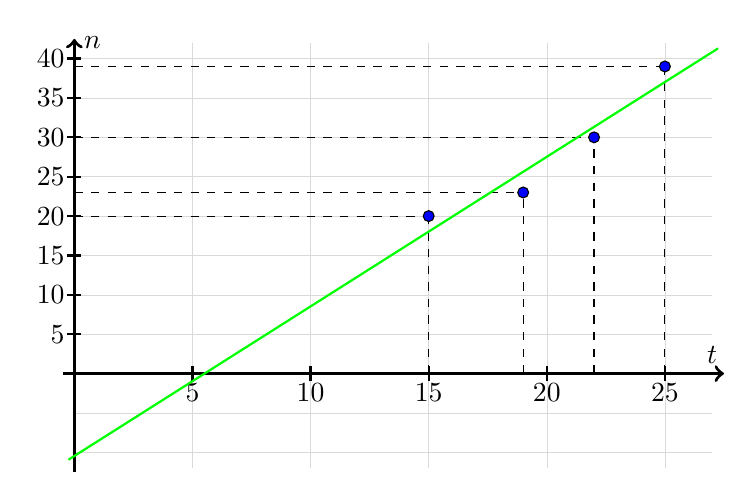
\begin{tikzpicture}[xscale=0.3, yscale=0.1]
	
	\def\a{1.8995}
	\def\b{-10.4649}
	\def\t{{15, 19, 22, 25}}
	\def\n{{20, 23, 30, 39}}


	%grid
	%\draw [very thin, draw=gray!30] (0,-12) grid (27,42);
	\foreach \i in {0, 5, ..., 25}
	{
		\draw [very thin, draw=gray!30] (\i, -12) -- (\i, 42);
	}
	\foreach \i in {-10, -5, ..., 40}
	{
		\draw [very thin, draw=gray!30] (0, \i) -- (27, \i);
	}
	
	%Achsen
	\draw [very thick, ->] (0, -12.5) -- (0, 42.5);
	\draw [very thick, ->] (-0.5, 0) -- (27.5, 0);
	\node [right] at (0, 42) {$n$};
	\node [above] at (27, 0) {$t$};
	\foreach \i in {5, 10, ..., 25}
	{
		\draw [thick] (\i, -1) -- (\i, 1);
		\node [below] at (\i,0) {$ \i $};
	}
	\foreach \i in {5, 10, ..., 40}
	{
		\draw [thick] (-0.3, \i) -- (0.3, \i);
		\node [left] at (0, \i) {$ \i $};
	}

	%Datenpunkte
	\foreach \i in {0, 1, 2, 3}
	{
		\draw [dashed] (0, \n[\i]) -- (\t[\i], \n[\i]);
		\draw [dashed] (\t[\i], 0) -- (\t[\i], \n[\i]);
		\filldraw [fill = blue] (\t[\i],\n[\i]) ellipse (0.23 and 0.69);
	}

	%Regressionsgerade
	\draw[domain=-0.25:27.25,smooth,variable=\x,green, thick] 
	plot ({\x},{\a*\x + \b});
	
	
	
\end{tikzpicture}
